\section{Extensions of the Basic Model}


The basic model presented in section (\ref{section:derivation:basic_model}) currently has the following limitations
\begin{enumerate}
\item Dynamical systems with complex eigenvalues are ill-defined
\item Only $2d$ of $N$ neurons have nontrivial dynamics. 
\item Network dynamics are inherently periodic and deterministic, not asynchronous. 
\end{enumerate}

We extend the basic model to address these limitations. 

\subsection{Dynamical Systems with Complex Eigenvalues}
Recall the basic self-coupled network equations:

$$
\dot{v}
= 
\begin{bmatrix}
\Lambda & 0
\\
0 & 0
\end{bmatrix}
v +
\begin{bmatrix}
S \left(\Lambda + I_d \right) S & 0
\\
0 & 0
\end{bmatrix}
  \rho 
+ \beta \tilde{c}  
  - 
 \begin{bmatrix}
S^2 & 0
\\
0 & 0
\end{bmatrix}
    \tilde{o},
$$

$$
\dot{\rho} = -\rho + \tilde{o},
$$

$$
\hat{y} = \begin{bmatrix}
S & 0
\end{bmatrix}
\rho.
$$


When the dynamical system $\dot{x} = Ax + Bc$ is oscillatory, the eigenvalues $\Lambda$ of $A=\mathcal{U} \, \Lambda \, \mathcal{U}^T$ are complex, implying $\dot{v}$ is a system of complex equations. Currently, all network quantities are only defined for real-values. Here we generalize the self-coupled network to complex vector space so that it is well defined when $A$ has complex eigenvalues.


\begin{enumerate}

\item \textbf{\textit{Complex Eigenvalues of $A \in \mathbf{R}^{d \times d}$ Imply $x \in \mathbf{C}^d$: }} 
The existence of complex eigenvalues implies that $x$ is an element of a complex vector space $\mathbf{C}^d$. The spectral theorem assumes as much when proving the existence of an eigendecomposition for $A = \mathcal{U} \Lambda \mathcal{U}^T$. If we otherwise restrict $x$ to $\mathbf{R}^d$, the eigendecomposition $A$ would exist i.f.f. $A$ was symmetric, i.e. $A = A^T$. 



\item \textbf{\textit{Complex Eigenvectors $\mathcal{U} \in \mathbf{C}^{d \times d}$ form a Rotating Basis in $d-$dimensional space.}} The self-coupled network is derived by a change of bases into the eigenvectors of $A = \mathcal{U} \Lambda \mathcal{U}^T$ for d-dimensional vectors, and into the right eigenvectors $V$ of $D = \mathcal{U}\begin{bmatrix} S & 0 \end{bmatrix} V^T$ for $N-$dimensional quantities. For complex $\Lambda$, the d-eigenvectors $\mathcal{U}_j$ have angular velocities specified by $\Im \Lambda_j$. To see why, consider the dynamical system

$$
\dot{x} = Ax, \hspace{4mm} x(0) = x_0.
$$

The solution to this dynamical system is given by its modal decomposition onto $\mathcal{U}_j$, the $j^{th}$ eigenvector of $A$ with eigenvalue $\Lambda_j$:

$$
x(t) = \sum_{j=1}^{d} \left(x_0^T \mathcal{U}_j\right) e^{i \Lambda_j t} \mathcal{U}_j.
$$

In modal decomposition, the initial state $x_0$ is expressed by projection onto each orthonormal eigenvector $\mathcal{U}_j$. The dynamics of an eigenvector are trivial: eigenvector $j$ is scaled in time by $e^{\Lambda_j t}$. This makes computing the projection dynamics  trivial. The solution $x(t)$ is the sum of the scaled eigenvector projections. 


When $\Lambda_j$ is complex, the scaling takes an angular velocity via Euler's relation

$$
e^{i \theta} = cos(\theta) + i \, sin(\theta).
$$

The angular velocity is the imaginary component of $\Lambda_j = \sigma_j + i \, \omega_j$: 

\begin{align*}
e^{i \Lambda_j \, t} 
&=
e^{\sigma_j \, t} e^{i \omega_j t}
\\
\\
&=
e^{\sigma_j \, t} \left(cos(\omega_j t) + i \, sin(\omega_j t)\right).
\end{align*}

In the self-coupled network, the eigenvectors $\mathcal{U}$ form the encoding directions for each neuron. Therefore, complex eigenvalues imply oscillatory encoding directions in the self coupled network, with angular frequency $\omega_j = \Im \Lambda_j$. 

 

\item \textbf{\textit{Real Spike Trains $\tilde{o} \in \mathbf{R}^d$ Imply $N = 2d$ Neurons Cannot Encode $\mathbf{C}^d$. $N = 4d$ Neurons Can.}} In the basic derivation, we doubled the number of neurons from $d$ to $2d$ because $d$ neurons could not encode a $d-$dimensional space by using spikes with strictly positive area $o(t)$. To extend to the case of complex encoding directions, we first formalize the argument for doubling in the basic network derivation. 









 Even lower than both of these is the unconstrained optimization, 
$$
\underset{\rho \in \mathbf{R}^{d}}{min} ||y - S \rho ||^2, 
$$

whose solution is 
$$
\rho^* = S^{-1}y. 
$$


\item\textbf{\textit{The Network Optimizes Spike Times by Comparing Against Real and Imaginary Voltage Thresholds Simultaneously.}}



Complex quantities are often simpler to manipulate in polar coordinates than Cartesian, so we use them here. For any complex scalar $\alpha \in \mathbf{C}$, the relation between polar and Cartesian coordinates is
$$
\alpha = a + i b = \mu e^{i \theta}, 
$$
where
\begin{align*}
\mu &= \sqrt{a^2 + b^2}, 
\\
\\
\theta &= \tan^{-1}\frac{b}{a},
\\
\\
a + ib &= \mu \, cos \,\theta + i \, \mu \,  sin \, \theta = e^{i\theta}.
\end{align*}

\item\textbf{\textit{Preferred Directions in $\mathbf{R}^d$ Cannot Encode vectors in $\mathbf{C}^d$}}

\item Let $\bar{\Lambda}$ denote the polar representation of $\Lambda$, the eigenvalues of $A$. 
$$
\bar{\Lambda}_j
\overset{\Delta}{=}
\mu_j \, e^{i \omega_j},
$$

where 

$$
\omega_j = tan^{-1} \frac{\Re\Lambda_j}{\Im\Lambda_j}, 
$$
and
$$
\mu_j = \sqrt{\Re\Lambda_j^2 + \Im\Lambda_j^2}.
$$

$A$'s eigenvalues are
$$
\Lambda = 
\begin{bmatrix}
\Lambda_1 & 0 & \hdots &0  & 0
\\
0 & \Lambda_2 & 0 & \hdots & 0
\\
\vdots & & & & \vdots
\\
 0& 0  & 0 & 0 & \Lambda_d
 \end{bmatrix}
 = 
 \begin{bmatrix}
\mu_1 \, e^{i \omega_1} & 0 & \hdots &0  & 0
\\
0 & \mu_2 \, e^{i \omega_2} & 0 & \hdots & 0
\\
\vdots & & & & \vdots
\\
 0& 0  & 0 & 0 & \mu_d \, e^{i \omega_d}
 \end{bmatrix} = \bar{\Lambda}.
$$

Transforming the eigenvector, we denote the $k^{th}$ complex component of $\mathcal{U}_j$ by $u_{kj}^\Re + i \, u_{kj}^\Im$. Let $W_j$ denote the polar representation of $\mathcal{U}_j$.

$$
\mathcal{U}_j 
=
\begin{bmatrix}
u_{1j}^\Re + i u_{1j}^\Im
\\
\vdots
\\
u_{dj}^\Re + i u_{dj}^\Im
\end{bmatrix}
=
\begin{bmatrix}
\alpha_{1j} e^{i \theta_{1j}}
\\
\vdots
\\
\alpha_{dj} e^{i \theta_{dj}}
\end{bmatrix} = W_j,
$$
where

$$
\alpha_{ij} = \sqrt{(u_{ij}^\Re)^2 + (u_{ij}^\Im)^2},
$$

and

$$
\theta_{ij} = tan^{-1} \frac{u_{ij}^\Im}{u_{ij}^\Re}.
$$


We now write $A$ as 
$$
A = 
W \bar{\Lambda} W^*.
$$

\item \textbf{\textit{Question:}} At time $\xi$ what is the minimum objective achievable by the network

$$
\mathcal{L}(\xi, S_j) = ||y - (\hat{y} + S_j)||,
$$

assuming we can add one of $W_j $ where $D = W \begin{bmatrix} S & 0 \end{bmatrix} V^T$ or nothing. 

\textbf{\textit{Hypothesis:}} The minimum objective is given by

$$
min \underset{x \in S \cup {0}}{\mathcal{L}}(\xi, x) = \mathcal{L}(\xi, x^*), 
$$

where 

$$
x^* = argmin \underset{x \in S \cup {0}}{\mathcal{L}}(\xi, x).
$$

\textbf{\textit{Experiment:}} Given a simple known-correct network, compute $x^*$ and $min(\mathcal{L})$ at each point in time. Compare this to network output.  
Specifically, number each choice for $x$ from $0, \ldots, d$, where $0$ is the zero vector. At each time step, the network chooses one of these vectors. Record this integer choice. Likewise, compute the hypothesized objective and record the integer output.  Compare the two data. If they are identical the hypothesis holds for the experiment. Otherwise, the network is \textit{not} performing the optimization. 

\textbf{\textit{Results:}}  The known network correctly spiked to reduce the error to its minimum possible. It was identical to the objective function shown.  

\textbf{\textit{Question:}} What is the smallest possible objective achievable by the network if it could add arbitrary combinations of its coding vectors to its estimate. Now what is it if we only allow integer combinations, 1 per timestep? 

\textbf{\textit{Hypothesis:}} The smallest possible objective achieved by arbitrary combinations of neurons encoding vectors is the least-squares solution

$$
\mathcal{L^*}_{\mathbf{C}} = \underset{x \in \mathbf{C}^N}{min}||y - \hat{y} + \begin{bmatrix} S & 0 \end{bmatrix} x||^2. 
$$

Restricting the domain of $x$ to real combinations of vectors will yield a greater error.

$$
\mathcal{L^*}_\mathbf{R} = \underset{x \in \mathbf{R}^N}{min}||y - \hat{y} + \begin{bmatrix} S & 0 \end{bmatrix} x||^2 \geq \mathcal{L^*}_{\mathbf{C}}.
$$


If we restrict to the domain of Gaussian Integers  $\mathbf{Z}^N[i]$(complex numbers with integer components), it is unclear whether the error is less than or greater than restricting to $\mathbf{R}^N$.
$$
\mathcal{L^*}_\mathbf{Z}[i] = \underset{x \in \mathbf{Z}^N[i]}{min}||y - \hat{y} + \begin{bmatrix} S & 0 \end{bmatrix} x||^2 \geq \mathcal{L^*}_{\mathbf{C}}.
$$


If we restrict to the domain of real integers , this will necessarily be larger than the preceding objectives:

$$
\mathcal{L^*}_\mathbf{Z} = \underset{x \in \mathbf{Z}^N[i]}{min}||y - \hat{y} + \begin{bmatrix} S & 0 \end{bmatrix} x||^2 \geq \mathcal{L^*}_{\mathbf{C}}.
$$


Finally we restrict the domain to a single vector multiple, which will always be the largest objective. This is the optimization performed by the network.  
$$
\mathcal{L^*}_\mathbf{1} = \underset{x \in \mathbf{Z}^N \, : \, \sum{Z_i} = 1}{min}||y - \hat{y} + \begin{bmatrix} S & 0 \end{bmatrix} x||^2 \geq \mathcal{L^*}_{\mathbf{Z}[i]}.
$$


\textbf{\textit{Experiment}}: For a given simulation, compute the objectives above at each timestep. Plot the minimum objectives versus time.  For a set of simulations, sweep the scaling of $D$ and record the average  of each minimum objective. Plot the scaling $D$ versus this average for each objective. The plots should test the above hypotheses.  





\clearpage





\item The given decoder matrix  $D$ maps integrated spikes from $\mathbf{R}^N$ to the network estimate $\hat{x} \in \mathbf{R}^d$. View $D = \mathcal{U} \begin{bmatrix}S & 0 \end{bmatrix} V^T$ as a sequence of linear maps between vector spaces as in figure (\ref{fig:linear_maps_between_subspaces_D_real}). For complex $\hat{x}$, we require that $D$ map from $\mathbf{C}^N$ to $\mathbf{C}^d$. By assumption, $D$ and $A$ share a common left basis, which is now $W \in \mathbf{C}^{d \times d}$. However the remaining real-valued matrices $S, V$ discard any complex components, limiting the span of $D$ to the complex basis $W$ scaled only by real coefficients, as in figure (\ref{fig:linear_maps_between_subspaces_D_complex}). To ensure that $D$ spans $\mathbf{C}^d$ and not a real-coefficient subspace, we extend $S$ and $V$ to the complex domain. Denote these complexified matrices by $\bar{S}$ and $\bar{V}$ respectively. 



\begin{figure}
\centering
\includegraphics[scale=.6]{figures/linear_map_sequence_complex}
\caption{$D$ projects vectors to $\mathbf{R}^d$ before expansion in the basis $W$. \textbf{\textit{Top: }} The matrix $D=W \begin{bmatrix} S & 0 \end{bmatrix} V^T$ shares a complex left-basis $W$ with $A$. However the remaining matrices $S$ and $V$ are real-valued. This limits the range of $D$ to real linear combinations of the basis $W$. \textbf{\textit{Bottom:}} We complexify $S \rightarrow \bar{S}$ and $V \rightarrow \bar{V}$ and rotate network quantities to the $W-\bar{V}$ basis. This ensures that the $span(D) = \mathbf{C}^d$.
}
\label{fig:linear_maps_between_subspaces_D_complex}
\end{figure}

\clearpage

A principled method of extending real functions in $\mathbf{R}^d$ to the complex plane $\mathbf{C}^d$ is to use the Hilbert Transform. Suppose our real function is $f(x)$ and we wish to find $g(x)$ such that $h(x) = f(x) + ig(x)$. The Hilbert transform of $f$ gives a $g$ such that $h$ has at least two useful properties. 1) $h(x)$ is complex-differentiable in $x$; 2) The Fourier transform of $h$ has no negative frequency components, which respects the conjugate-symmetric spectrum of the real-valued $f$. 

Let $H_x(f)$ denote the Hilbert Transform of the function $f$ over the domain $x$, i.e. 

$$
H_x(f) \overset{\Delta}{=} \frac{1}{\pi} \int_{-\infty}^{\infty} \frac{f(y)}{x - y} dy
=
f * \frac{1}{\pi x} (x). 
$$

We complexify the matrix $D$ by applying the Hilbert transform to the columns of $S$ and of $V$ over the domain $k \in \left[ 1,\hdots,d\right]$;  i.e
$$
\bar{S} = 
\begin{bmatrix}
H_k(S_1) & \hdots & H_k(S_d)
\end{bmatrix}  
= H_k(S),
$$

$$
\bar{V} = 
\begin{bmatrix}
H_k(V_1) & \hdots & H_k(V_N)
\end{bmatrix}  
= H_k(V).
$$

Here $k \in \mathbf{Z}$ is a discrete domain of indices, so we use the discrete version of the Hilbert transform.


\item The neurons which implement the network have spike trains $\tilde{o}(\xi) \in \mathbf{C}^{N}$:
    \begin{equation*}
        \tilde{o}_j(\xi) = \sum_{k=1}^{\text{$n_j$ spikes}} \delta(\xi - \xi_{j}^{k}) + i0,
    \end{equation*}
	which have no imaginary component. 
	
    The network's estimate is
	$$
      \hat{y}(\xi) = \begin{bmatrix}
      \bar{S} & 0
      \end{bmatrix} \rho(\xi), 
	$$
    for $\rho = \bar{V}^T r \in \mathbf{C}^N$ where
	$$
        \frac{d\rho}{d \xi} = -\rho + o(\xi).
    $$
	The network error $\epsilon \in \mathbf{C}^d$ is 
	$$
		\epsilon = y - \hat{y}  = W^* e.
	$$


\item Before deriving the network voltage dynamics, we redefine voltage as complex using network optimization. Consider the previous optimization from which voltage was defined
$$
\mathcal{L} = || y(\xi + d\xi) - \hat{y}(\xi + d\xi)||^2 = \epsilon^T \epsilon \in \mathbf{R}.$$

The network optimized the Euclidean norm of two real vectors given by the inner product of the error with itself. We generlize to complex vectors by using the complex inner product. I.e, 

$$
\mathcal{L}(\xi) = \epsilon^*\epsilon, 
$$
where $*$ denotes the Hermitian transpose.

When neuron $j$ does not spike, the objective is

\begin{align*}
\mathcal{L}_{ns} 
&= \epsilon^*\epsilon = \sum_{j=1}^d \Re\left\{\epsilon_j\right\}^2 + \Im\left\{\epsilon_j\right\}^2
\end{align*}


When neuron $j$ spikes, the vector $\bar{S}_j$ is added to the network estimate so that the objective is

\begin{align*}
\mathcal{L}_{sp}
&=
(y - \hat{y} - \bar{S}_j)^*(y - \hat{y} - \bar{S}_j)
\\
\\
&=
\left(\epsilon-\bar{S}_j\right)^*\left(\epsilon-\bar{S}_j\right)
\\
\\
&=
\epsilon^*\epsilon  - \epsilon^*\bar{S}_j - \bar{S}_j^*\epsilon + \bar{S}_j^*\bar{S}_ja
\\
\\
&=
\mathcal{L}_{ns} - \left(\bar{S}_j^*\epsilon\right)^* - \bar{S}_j^* \epsilon + ||\bar{S}_j||^2 
\\
\\
&=
\mathcal{L}_{ns} - \left[\left(\bar{S}_j^*\epsilon\right)^* + \bar{S}_j^* \epsilon\right] + ||\bar{S}_j||^2 
\end{align*}

The middle two terms in brackets sum a complex number $\bar{S}_j^* \epsilon$  and its conjugate. For any complex scalar $c = a + ib$, the sum with its conjugate is $c + c^* = (a + ib) + (a - ib) = 2a$.

It follows that 

$$
\mathcal{L}_{sp} = \mathcal{L}_{ns} - 2 \Re \left[\bar{S}_j^*\epsilon\right] + ||\bar{S}_j||^2.
$$

The spiking condition $\mathcal{L}_{sp} < \mathcal{L}_{ns}$ is then
$$
\Re \left[\bar{S_j}^*\epsilon\right] > \frac{\bar{S}_j^* \bar{S}_j}{2}.
$$

Using the same argument as in the basic derivation, the voltage for complex-eigenvalued $A$ is defined as the $ReLu$ of the above quantity. 

$$
v_j \overset{\Delta}{=} ReLu\left(\Re \left[\bar{S}_j^*\epsilon\right] \right).
$$

The spike rule then becomes, i.e
$$
v_j > \frac{||\bar{S}_j||^2}{2}.
$$


Simulating the network as described above produces the following:

TODO: Insert FIgure of degenerate network sim here

The performance is poor. To see why, note that the spiking condition does not depend on the imaginary component of neuron $j$'s voltage, meaning that multiple neuron's wit  


\clearpage

\item We now derive the voltage dynamics as before. The rotated target dynamical system is

$$
\dot{y} = \bar{\Lambda} y + \beta \tilde{c},
$$

where 
$$
\beta = W^* B W,
$$

$$
\tilde{c} = W^* c.
$$

The error has dynamics

\begin{align*}
\dot{\epsilon} &= \dot{y} - \dot{\hat{y}}
\\
\\
&=
\bar{\Lambda}y + \beta \tilde{c} - \begin{bmatrix}
S & 0
\end{bmatrix}
\dot{\rho}
\\
\\
&= 
\bar{\Lambda}y + \beta \tilde{c}
+
\begin{bmatrix}
S & 0
\end{bmatrix}
\rho
-
\begin{bmatrix}
S & 0
\end{bmatrix}
\tilde{o}.
\end{align*}


Apply the matrix $\begin{bmatrix}
\bar{S} \\ 0
\end{bmatrix}^*$ to both sides and take the real part to get the voltage dynamics. We write the full set of $N$ equations as
$$
\dot{v} = 
\begin{bmatrix}
\bar{\Lambda} & 0 \\ 0 & 0
\end{bmatrix}
v
+
\begin{bmatrix}
\bar{S}^*\left(I + \bar{\Lambda}\right) \bar{S}  & 0 \\ 0 & 0
\end{bmatrix} \rho 
+
\beta \tilde{c}
-
\begin{bmatrix}
\bar{S}^* \bar{S} &  0 \\ 0 & 0
\end{bmatrix} \tilde{o}.
$$

\end{enumerate}

To summarize, the self-coupled network model is extended to complex-valued dynamical systems by the following:
\begin{enumerate}
	\item Factorize $A = \mathcal{U}\Lambda\mathcal{U}^T$, by assumption $\Lambda$ contains complex entries. Rewrite this matrix as $A = W^T \bar{\Lambda} W$ so that $\bar{\Lambda}$ contains only real entries.
	
	\item The voltage contains the sum of real and imaginary components of the error projected onto the rotated (now complex) basis $W$. 
	
	\item 
\end{enumerate}



\clearpage

Suppose the following definitions:

$$\epsilon \overset{\Delta}{=} y - \hat{y}$$

$$ V \overset{\Delta}{=} \begin{bmatrix}
S \\ 0
\end{bmatrix} \epsilon.
$$

Conjecture: There is no lower bound on voltage $v$ and the definitions above are both true at the same time.  
\\
\\
Counterexample: Consider the  one-dimensional system:
$$
\Lambda = -I =  -1 
$$

$$
\beta = I = 1
$$

$$
S = [1, -1] \implies v_{th} = \frac{1}{2}
$$

$$
N = 2.
$$

$$
c(t) = 2
$$

Solve the system explicitly using voltage dynamics and firing rate equations. 

Neuron A: 

$$
\dot{v_A} = -v_A + 2, \, \, \, v_A(0) = 0
$$
\\
\\
$$
v_A(t) \text{ spikes at rate } \phi \simeq 2 \text{ Hz}
$$



Neuron B:
$$
\dot{v_B} = -v_B - 2, \, \, \, v_B(0) = 0
$$

$$
v_B(t) = 2 e^{-t} -2,
$$

$$
v_B(10)  \simeq -2 = - 4 \, v_{th}.
$$


Error:

$$
y(t) = 2 - 2 e^{-t}, \, \, \, y(0) = 0
$$

$$
y(10) \simeq 2.
$$


$$
\hat{y}(t) = \frac{1}  {1 - e^{-\frac{1}{2}}}  e^{-t \, mod \, \frac{1}{2}} = 2 \pm \frac{1}{2}.
$$

$$
\epsilon = y - \hat{y}  < v_{th} = \frac{1}{2}.
$$

From definition of voltage, 

$$
v_A = \epsilon < \frac{1}{2}
$$

$$
v_B = -\epsilon \implies -\frac{1}{2} < v_B < 0.
$$

However $v_B(10) < -\frac{1}{2}$, which is a contradiction. 


\clearpage





















